% Docs in  http://www.tex.ac.uk/ctan/macros/latex/contrib/memoir/memman.pdf

\newcommand{\mytitle}{Sample Statement of Work}
\newcommand{\mysubtitle}{Every document needs a subtitle...}
\newcommand{\mybody}{\pagebreak

\hyperdef{}{}{\section{Background}}

Every project needs a background. Here's some lorem ipsum about the project.

Lorem ipsum dolor sit amet, consectetur adipiscing elit. Nulla sit amet arcu elit. Donec at massa et leo auctor fringilla vitae id erat. Nam feugiat velit vitae ornare tristique. Morbi porttitor, orci vel dapibus malesuada, magna libero ultrices massa, nec interdum diam nisi elementum ipsum. Vestibulum elit lorem, pretium id semper ac, aliquam ut dui. Etiam at magna non nibh viverra tristique. Maecenas consectetur vulputate tellus, ac rutrum felis molestie ut. Aenean tincidunt congue cursus. Maecenas in egestas magna, nec pellentesque justo. Phasellus ante quam, faucibus sit amet tellus et, fringilla convallis eros.

Nullam vitae imperdiet enim. Ut id ultrices leo. In dictum bibendum vestibulum. Donec lobortis condimentum mauris ac interdum. Duis bibendum molestie eleifend. Nunc non neque a neque ornare euismod non ut sapien. Morbi sed diam quis felis commodo vehicula ac et augue. Maecenas pretium justo sit amet imperdiet pharetra.

Nunc at odio massa. In hac habitasse platea dictumst. Donec posuere erat ac ultrices suscipit. Quisque id velit nulla. Ut in urna orci. Sed at euismod neque. Sed velit velit, fringilla vitae eleifend eget, auctor id mi.

\pagebreak

\hyperdef{}{}{\section{Proposed Solution}}

This wouldn't be a proposal unless it proposed something. We will re-architect the system into a series of robust robust components:

\begin{enumerate}
\itemsep1pt\parskip0pt\parsep0pt
\item
  export, a script to export the data from access, validate it, refactor it into a logical format, then output it in plain-text format.
\item
  import, a simple, robust module to handle file uploads of the cleaned data, and efficiently import this data. It will do sufficient error handling to allow full automation.
\end{enumerate}

As we perform the refactoring, we will rewriting the code to ensure it's documented, easy to test, and easy to update as future needs are identified.

\hyperdef{}{}{\subsection{Export component}}

\begin{itemize}
\itemsep1pt\parskip0pt\parsep0pt
\item
  This will be a standalone script responsible for extracting data from source database, and cleaning it up as appropriate.
\item
  The output format is human readable JSON files, with a logical, easy to understand structure
\item
  Easy to verify output through manual inspection of output
\item
  Include comprehensive automated tests to ensure output is correct
\end{itemize}

\hyperdef{}{}{\subsection{Import component}}

\begin{itemize}
\itemsep1pt\parskip0pt\parsep0pt
\item
  Allows non-technical staff to upload already validated JSON files, and sync the target database accordingly.
\item
  Assumes that input data is relatively safe, as it's produced via the export component
\item
  Will be optimized to perform quickly; typical runs will be completed within 60 seconds
\item
  Improved validation and error handling
\end{itemize}

\hyperdef{}{}{\subsection{Benefits of our solution}}

Here's some more \textbf{lorem ipsum}~for you all. Nullam vitae imperdiet enim. Ut id ultrices leo. In dictum bibendum vestibulum. Donec lobortis condimentum mauris ac interdum. Duis bibendum molestie eleifend. Nunc non neque a neque ornare euismod non ut sapien. Morbi sed diam quis felis commodo vehicula ac et augue. Maecenas pretium justo sit amet imperdiet pharetra.

Nunc at odio massa. In hac habitasse platea dictumst. Donec posuere erat ac ultrices suscipit. Quisque id velit nulla. Ut in urna orci. Sed at euismod neque. Sed velit velit, fringilla vitae eleifend eget, auctor id mi.

Nullam vitae imperdiet enim. Ut id ultrices leo. In dictum bibendum vestibulum. Donec lobortis condimentum mauris ac interdum. Duis bibendum molestie eleifend. Nunc non neque a neque ornare euismod non ut sapien. Morbi sed diam quis felis commodo vehicula ac et augue. Maecenas pretium justo sit amet imperdiet pharetra.

Nullam vitae imperdiet enim. Ut id ultrices leo. In dictum bibendum vestibulum. Donec lobortis condimentum mauris ac interdum. Duis bibendum molestie eleifend. Nunc non neque a neque ornare euismod non ut sapien. Morbi sed diam quis felis commodo vehicula ac et augue. Maecenas pretium justo sit amet imperdiet pharetra.

\pagebreak

\hyperdef{}{}{\section{Schedule and Budget}}

The work described in this mandate will take 300 hours to complete, to be performed within 6-8 weeks of the signing of this agreement.

\hyperdef{}{}{\subsection{Table}}

Here is a schedule of the work:

\hyperref[]{}\hyperref[]{}

\begin{longtable}[c]{@{}ll@{}}
\toprule\addlinespace
\begin{minipage}[t]{0.47\columnwidth}\raggedright
gdocs-export:author
\end{minipage} & \begin{minipage}[t]{0.47\columnwidth}\raggedright
Alex
\end{minipage}
\\\addlinespace
\begin{minipage}[t]{0.47\columnwidth}\raggedright
1
\end{minipage} & \begin{minipage}[t]{0.47\columnwidth}\raggedright
150
\end{minipage}
\\\addlinespace
\begin{minipage}[t]{0.47\columnwidth}\raggedright
2
\end{minipage} & \begin{minipage}[t]{0.47\columnwidth}\raggedright
150
\end{minipage}
\\\addlinespace
\bottomrule
\end{longtable}

The following diagram should be on a separate page, to test page break:

\pagebreak

\hyperdef{}{}{\subsection{Diagram showing how work is split}}

Every document needs a diagram!

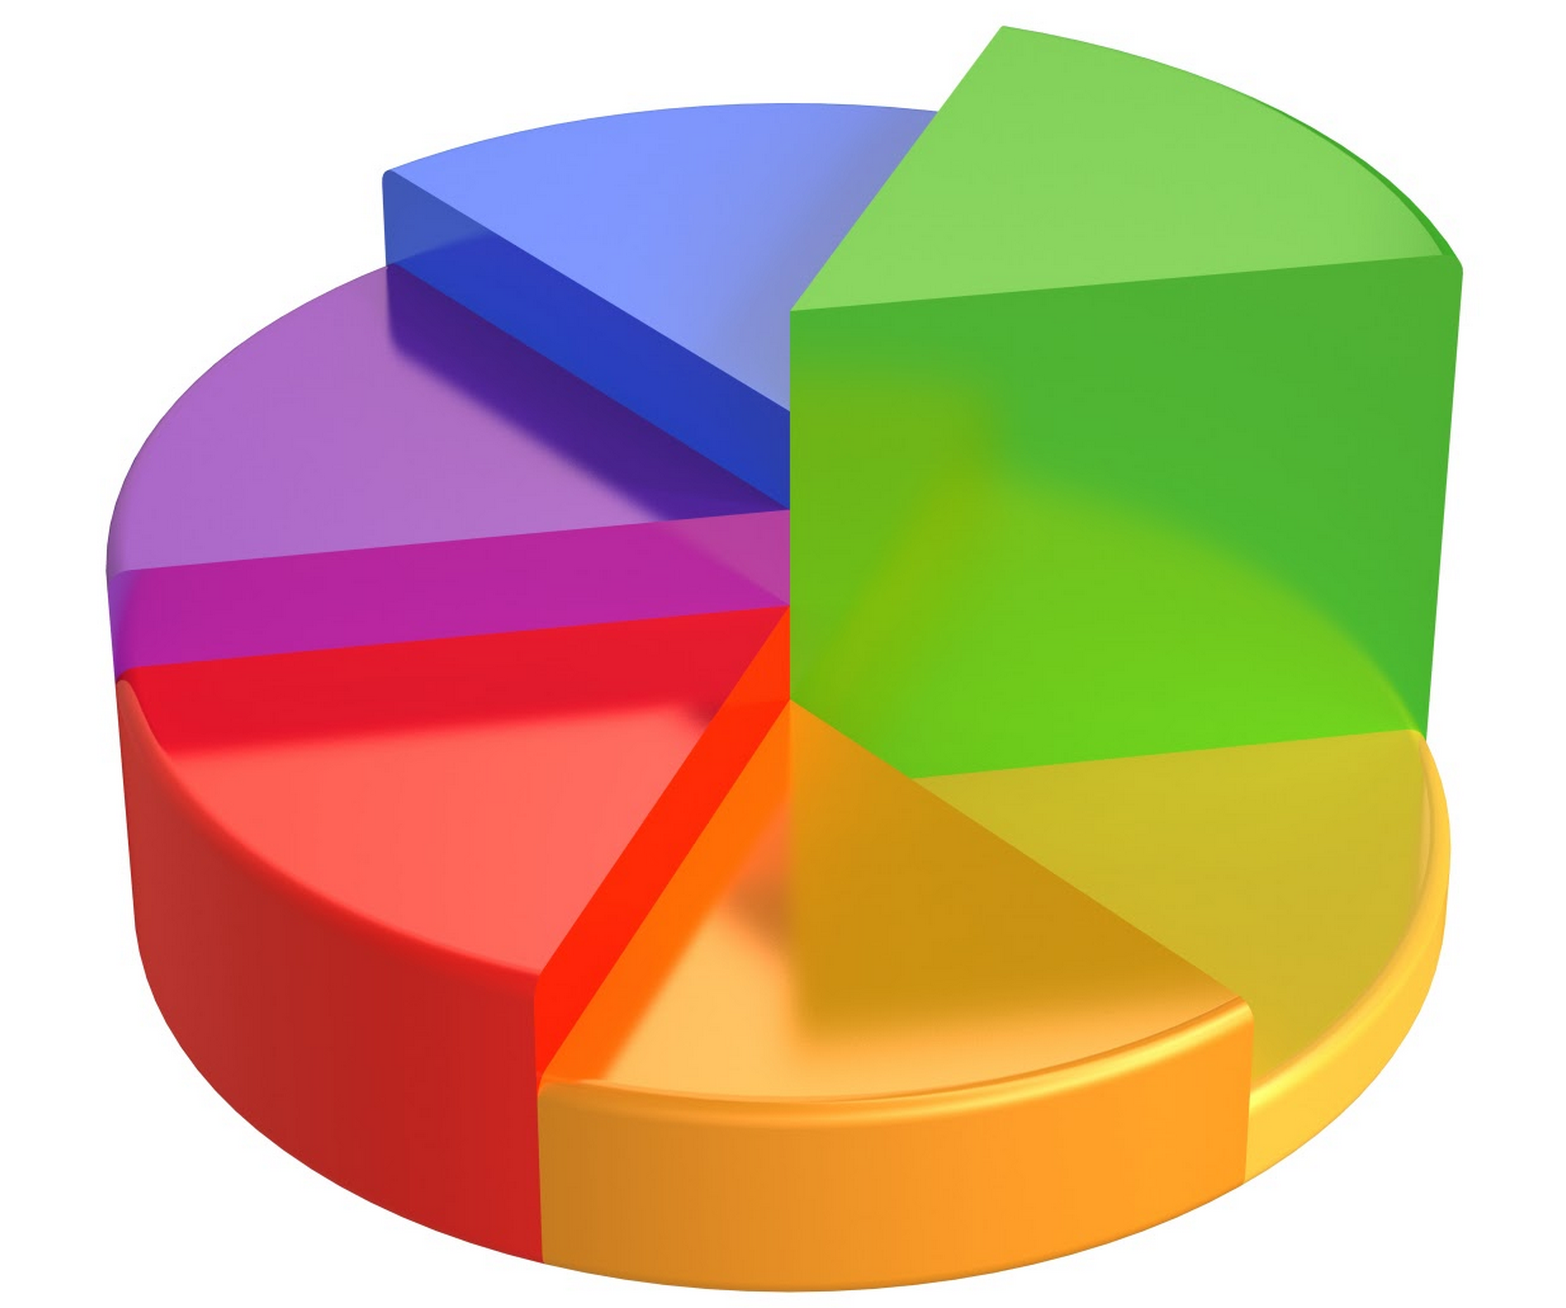
\includegraphics{SHbO80B3zYiLwN09wcE1jxTyLWaBsr7llKXblVz0EwCQsT2EsGznwPa4YwxgN3BwyMSEZhyazyYEoA5TNEBswNe6FJ2ZZsw9_E5R3YnzdCYFfcxjoR-rnHg.jpg}

\pagebreak

\hyperdef{}{}{\section{Terms and Conditions}}

\hyperdef{}{}{\subsection{Staffing}}

Appropriate staff will be used for the execution of this project.

\hyperdef{}{}{\subsection{Relation to Other Agreements}}

This agreement is governed by the same terms and conditions as some other documents.

\hyperdef{}{}{\subsection{Language of Contract}}

Les parties ont convenu de rédiger cette entente en anglais. Parties have decided that this agreement be formulated in English.

\pagebreak

\hyperdef{}{}{\section{Agreement}}

This document is a contract, and contracts must be signed.

Signed on behalf of \textbf{Client LLC}:

~

~

\hrulefill

Name and title

~

~

\hrulefill

Signature and date

Signed by Adam Smith, President of \textbf{Vendor Inc.:}

\hrulefill

Signature and date}


% TODO: support table of key-value metadata in google doc


\documentclass[letterpaper,oldfontcommands,11pt,extrafontsizes,onecolumn,oneside,openboth,final,titlepage]{memoir}
\usepackage[T1]{fontenc}
\usepackage{lmodern}
\usepackage{amssymb,amsmath}
\usepackage{ifxetex,ifluatex}
\usepackage{fixltx2e} % provides \textsubscript

% reduce page margins to a reasonable size
\setlrmarginsandblock{2.5cm}{2.5cm}{*}
\setulmarginsandblock{2.5cm}{2.5cm}{*}
\checkandfixthelayout


% use microtype if available
\IfFileExists{microtype.sty}{\usepackage{microtype}}{}
% use upquote if available, for straight quotes in verbatim environments
\IfFileExists{upquote.sty}{\usepackage{upquote}}{}

\usepackage[utf8]{inputenc}
\usepackage{eurosym}

% http://tex.stackexchange.com/questions/37868/fancyhdr-and-memoir
\let\footruleskip\undefined

\usepackage{fancyhdr}
\renewcommand{\headrulewidth}{0pt}

% Chapter 2. Project Description ==> 2. Project Description
\renewcommand{\chaptermark}[1]{\markboth{\thechapter.\ #1}{}}

\fancypagestyle{plain}{  % used for pages that start new chapters
  \lhead{}
  \chead{}
  \rhead{}
  \cfoot{}
  \rfoot{\thepage/\thelastpage}
}

\fancypagestyle{gdocs}{
  \lhead{}
  \chead{}
  \rhead{\itshape{\nouppercase{\leftmark}}}
  \cfoot{}
  \rfoot{\thepage/\thelastpage}
}

\pagestyle{gdocs}

\chapterstyle{komalike} % also consider article, tandh


% used for printing google docs templates
\usepackage{longtable}
% used for printing google docs images
\usepackage{graphicx}
% We will generate all images so they have a width \maxwidth. This means
% that they will get their normal width if they fit onto the page, but
% are scaled down if they would overflow the margins.
\makeatletter
\def\maxwidth{\ifdim\Gin@nat@width>\linewidth\linewidth
\else\Gin@nat@width\fi}
\makeatother
\let\Oldincludegraphics\includegraphics
\renewcommand{\includegraphics}[1]{\Oldincludegraphics[width=\maxwidth]{#1}}

% used for google docs links
\usepackage[unicode=true]{hyperref}
\hypersetup{breaklinks=true,
            bookmarks=true,
            pdfauthor=, %TODO: fix the author
            pdftitle=\mytitle,
            colorlinks=true,
            urlcolor=blue,
            linkcolor=magenta,
            pdfborder={0 0 0}}

% Uncommnet to make embedded links print out HREF in footnotes, good for printing
% \renewcommand{\href}[2]{#2\footnote{\url{#1}}}

\setlength{\parindent}{0pt}
\setlength{\parskip}{7pt plus 2pt minus 1pt}
\setlength{\emergencystretch}{3em}  % prevent overfull lines

% Limits depth of automatic numbering of headings.
% 0 => Only H1 (chapters), 1 => Up to H2 (sections), 2 => Up to H3 (subsections)
\setcounter{secnumdepth}{2}

% memoir specific variable that lowers the title by 200pt
\setlength{\droptitle}{200pt}

% customize size and alignment of title and subtitle
\pretitle{\begin{flushleft}}
\title{\bfseries \HUGE \mytitle \\ \vskip .5em \LARGE \mysubtitle}
\posttitle{\par\vskip1em{\normalfont\normalsize\scshape \par\vfill}\end{flushleft}\vskip 0.5em}

% TODO generate the author somehow
% \author{}

% Suppress printing todays date.
% TODO: currently looks bad if not blank; make it look good and replace with todays date
\date{}

\begin{document}

\begin{titlingpage}
  \maketitle
  \vfill
  \Oldincludegraphics[width=3in]{./UNlogo.png}
\end{titlingpage}

\pagebreak

\textbf{Prepared by:}

Vendor Inc.,\\49 Seven square\\Montreal, QC H0H 0H0\\phone: (514)
345-6789\\fax: (514) 345-6789\\http://vendor.com

\textbf{}

\textbf{Prepared for:}

Client LLC,\\37 Prime Lane\\Montreal, QC H0H 0H0\\phone: (514)
345-6789\\fax: (514) 345-6789\\http://supplier.com

\vfill

CONFIDENTIAL: The contents of this document are confidential and are
intended exclusively for the designated recipients. The contents of this page
is defined in a file called sample-header.tex. Other legal mumbo jumbo\ldots{}.

\pagebreak


\setcounter{tocdepth}{1}
\begin{KeepFromToc}
  \hypersetup{linkcolor=black}
  \tableofcontents
\end{KeepFromToc}
\pagebreak

\pagebreak

\hyperdef{}{}{\chapter{Background}}

Every project needs a background. Here's some lorem ipsum about the project.

Lorem ipsum dolor sit amet, consectetur adipiscing elit. Nulla sit amet arcu elit. Donec at massa et leo auctor fringilla vitae id erat. Nam feugiat velit vitae ornare tristique. Morbi porttitor, orci vel dapibus malesuada, magna libero ultrices massa, nec interdum diam nisi elementum ipsum. Vestibulum elit lorem, pretium id semper ac, aliquam ut dui. Etiam at magna non nibh viverra tristique. Maecenas consectetur vulputate tellus, ac rutrum felis molestie ut. Aenean tincidunt congue cursus. Maecenas in egestas magna, nec pellentesque justo. Phasellus ante quam, faucibus sit amet tellus et, fringilla convallis eros.

Nullam vitae imperdiet enim. Ut id ultrices leo. In dictum bibendum vestibulum. Donec lobortis condimentum mauris ac interdum. Duis bibendum molestie eleifend. Nunc non neque a neque ornare euismod non ut sapien. Morbi sed diam quis felis commodo vehicula ac et augue. Maecenas pretium justo sit amet imperdiet pharetra.

Nunc at odio massa. In hac habitasse platea dictumst. Donec posuere erat ac ultrices suscipit. Quisque id velit nulla. Ut in urna orci. Sed at euismod neque. Sed velit velit, fringilla vitae eleifend eget, auctor id mi.

\pagebreak

\hyperdef{}{}{\chapter{Proposed Solution}}

This wouldn't be a proposal unless it proposed something. We will re-architect the system into a series of robust robust components:

\begin{enumerate}
\itemsep1pt\parskip0pt\parsep0pt
\item
  export, a script to export the data from access, validate it, refactor it into a logical format, then output it in plain-text format.
\item
  import, a simple, robust module to handle file uploads of the cleaned data, and efficiently import this data. It will do sufficient error handling to allow full automation.
\end{enumerate}

As we perform the refactoring, we will rewriting the code to ensure it's documented, easy to test, and easy to update as future needs are identified.

\hyperdef{}{}{\section{Export component}}

\begin{itemize}
\itemsep1pt\parskip0pt\parsep0pt
\item
  This will be a standalone script responsible for extracting data from source database, and cleaning it up as appropriate.
\item
  The output format is human readable JSON files, with a logical, easy to understand structure
\item
  Easy to verify output through manual inspection of output
\item
  Include comprehensive automated tests to ensure output is correct
\end{itemize}

\hyperdef{}{}{\section{Import component}}

\begin{itemize}
\itemsep1pt\parskip0pt\parsep0pt
\item
  Allows non-technical staff to upload already validated JSON files, and sync the target database accordingly.
\item
  Assumes that input data is relatively safe, as it's produced via the export component
\item
  Will be optimized to perform quickly; typical runs will be completed within 60 seconds
\item
  Improved validation and error handling
\end{itemize}

\hyperdef{}{}{\section{Benefits of our solution}}

Here's some more \textbf{lorem ipsum}~for you all. Nullam vitae imperdiet enim. Ut id ultrices leo. In dictum bibendum vestibulum. Donec lobortis condimentum mauris ac interdum. Duis bibendum molestie eleifend. Nunc non neque a neque ornare euismod non ut sapien. Morbi sed diam quis felis commodo vehicula ac et augue. Maecenas pretium justo sit amet imperdiet pharetra.

Nunc at odio massa. In hac habitasse platea dictumst. Donec posuere erat ac ultrices suscipit. Quisque id velit nulla. Ut in urna orci. Sed at euismod neque. Sed velit velit, fringilla vitae eleifend eget, auctor id mi.

Nullam vitae imperdiet enim. Ut id ultrices leo. In dictum bibendum vestibulum. Donec lobortis condimentum mauris ac interdum. Duis bibendum molestie eleifend. Nunc non neque a neque ornare euismod non ut sapien. Morbi sed diam quis felis commodo vehicula ac et augue. Maecenas pretium justo sit amet imperdiet pharetra.

Nullam vitae imperdiet enim. Ut id ultrices leo. In dictum bibendum vestibulum. Donec lobortis condimentum mauris ac interdum. Duis bibendum molestie eleifend. Nunc non neque a neque ornare euismod non ut sapien. Morbi sed diam quis felis commodo vehicula ac et augue. Maecenas pretium justo sit amet imperdiet pharetra.

\pagebreak

\hyperdef{}{}{\chapter{Schedule and Budget}}

The work described in this mandate will take 300 hours to complete, to be performed within 6-8 weeks of the signing of this agreement.

\hyperdef{}{}{\section{Table}}

Here is a schedule of the work:

\hyperref[]{}\hyperref[]{}

\begin{longtable}[c]{@{}ll@{}}
\toprule\addlinespace
\begin{minipage}[t]{0.47\columnwidth}\raggedright
gdocs-export:author
\end{minipage} & \begin{minipage}[t]{0.47\columnwidth}\raggedright
Alex
\end{minipage}
\\\addlinespace
\begin{minipage}[t]{0.47\columnwidth}\raggedright
1
\end{minipage} & \begin{minipage}[t]{0.47\columnwidth}\raggedright
150
\end{minipage}
\\\addlinespace
\begin{minipage}[t]{0.47\columnwidth}\raggedright
2
\end{minipage} & \begin{minipage}[t]{0.47\columnwidth}\raggedright
150
\end{minipage}
\\\addlinespace
\bottomrule
\end{longtable}

The following diagram should be on a separate page, to test page break:

\pagebreak

\hyperdef{}{}{\section{Diagram showing how work is split}}

Every document needs a diagram!

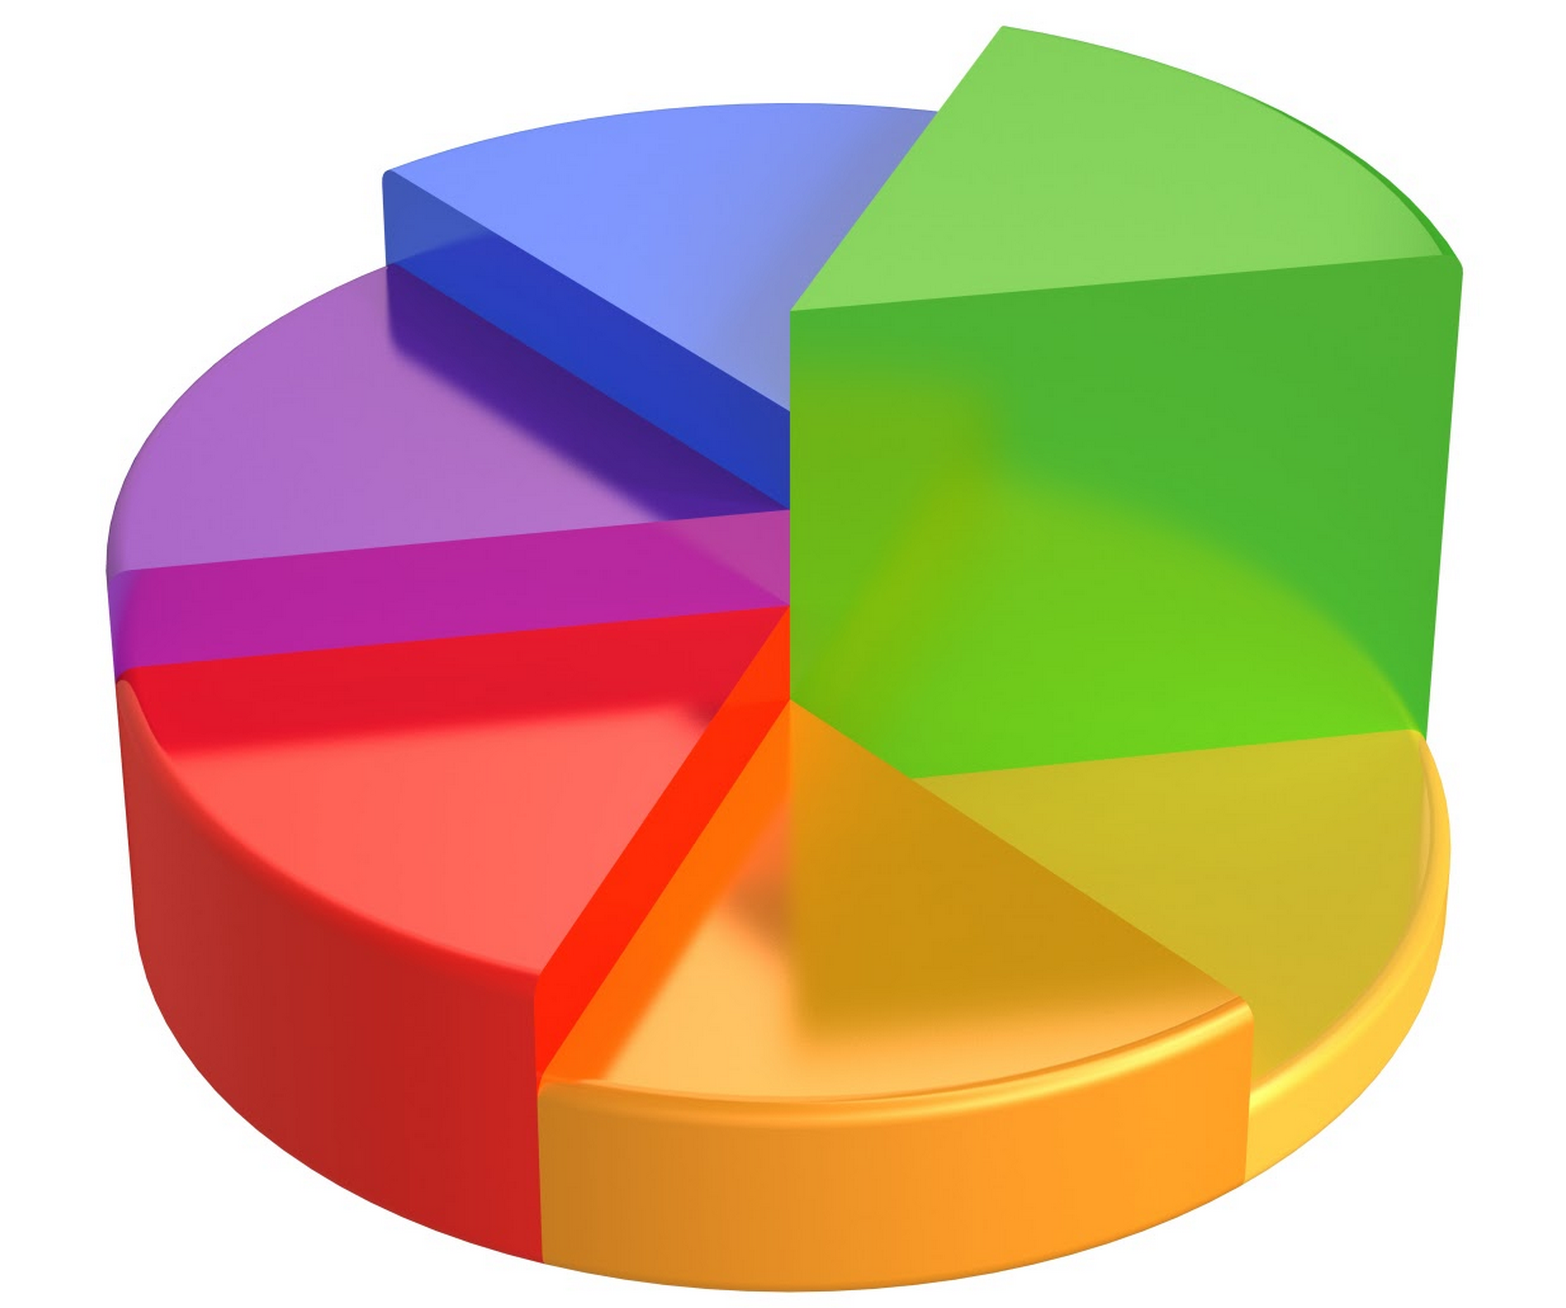
\includegraphics{SHbO80B3zYiLwN09wcE1jxTyLWaBsr7llKXblVz0EwCQsT2EsGznwPa4YwxgN3BwyMSEZhyazyYEoA5TNEBswNe6FJ2ZZsw9_E5R3YnzdCYFfcxjoR-rnHg.jpg}

\pagebreak

\hyperdef{}{}{\chapter{Terms and Conditions}}

\hyperdef{}{}{\section{Staffing}}

Appropriate staff will be used for the execution of this project.

\hyperdef{}{}{\section{Relation to Other Agreements}}

This agreement is governed by the same terms and conditions as some other documents.

\hyperdef{}{}{\section{Language of Contract}}

Les parties ont convenu de rédiger cette entente en anglais. Parties have decided that this agreement be formulated in English.

\pagebreak

\hyperdef{}{}{\chapter{Agreement}}

This document is a contract, and contracts must be signed.

Signed on behalf of \textbf{Client LLC}:

~

~

\hrulefill

Name and title

~

~

\hrulefill

Signature and date

Signed by Adam Smith, President of \textbf{Vendor Inc.:}

\hrulefill

Signature and date


\end{document}
